\documentclass{beamer}
\mode<presentation>
{
  \usecolortheme{seagull}
  \usetheme{Madrid}
}
\usepackage[english]{babel}
\usepackage{fontspec}
\usepackage{xunicode}
\usepackage{xltxtra}
\usepackage{url}
\setromanfont[Mapping=tex-text]{DejaVu Serif}
\setsansfont[Mapping=tex-text]{DejaVu Sans}
\setmonofont[Mapping=tex-text]{DejaVu Sans Mono}

\title[Android Resources]{Resources on Android}

\author{Mike Castleman}
\institute{Meetup}
\date[DevFest 2013]{ADI DevFest, 2013-02-04}

\pgfdeclareimage[height=0.5cm]{meetup-logo}{meetup-logo}
\logo{\pgfuseimage{meetup-logo}}

\begin{document}

\begin{frame}
  \titlepage
\end{frame}

\begin{frame}{Fragmentation}
\Large{``Developing for Android is hard, because there are lots of different
devices, and you have to test your app on every single one of them.''
\vskip 3em
--- People who never develop for Android}
\end{frame}

\begin{frame}{Four ``Abstract Densities''}
\begin{itemize}
\item \texttt{ldpi}: 75\% of base
\item \texttt{mdpi}: base image size (iOS ``1x'')
\item \texttt{hdpi}: 150\% of base
\item \texttt{xhdpi}: 200\% of base (iOS ``2x'')
\end{itemize}
\begin{tabular}{cccc}

\includegraphics[scale=0.5]{jogdial_l.png} &

\includegraphics[scale=0.5]{jogdial_m.png} &

\includegraphics[scale=0.5]{jogdial_h.png} &

\includegraphics[scale=0.5]{jogdial_xh.png} \\
\texttt{ldpi} & \texttt{mdpi} & \texttt{hdpi} & \texttt{xhdpi} \\
48×48 & 64×64 & 96×96 & 128×128
\end{tabular}
\end{frame}

\begin{frame}{Measurement Units}
\begin{itemize}
\item \texttt{px} --- physical device pixels
\item \texttt{dp} --- ``density-independent pixel''
\end{itemize}
On \texttt{mdpi}, 1 px = 1 dp. Not so on other densities!

Devices vary both in their density and in their size in dp.
\end{frame}

\begin{frame}{Examples}

\begin{itemize}
\item Phones
\begin{itemize}
\item HTC G1: 480x320px, \texttt{mdpi} = 480x320dp (medium, notlong)
\item Motorola Droid: 854x480px, \texttt{hdpi} = 570x320dp (medium, long)
\item Samsung Dart: 320x240px, \texttt{ldpi} = 427x320dp (small, notlong)
\item Galaxy Nexus: 1280x720px, \texttt{xhdpi} = 640x360dp (medium,
  long)
\end{itemize}
\item Tablets
\begin{itemize}
\item Kindle Fire: 1024x600px, \texttt{mdpi} = 1024x600dp (large)
\item Motorola Xoom: 1280x800px, \texttt{mdpi} = 1280x800dp (xlarge)
\end{itemize}
\end{itemize}
\end{frame}

\begin{frame}{But!}
\begin{itemize}
\item Android will automatically scale if you don't have appropriate
  files.
\item \texttt{ldpi} maybe irrelevant.\\
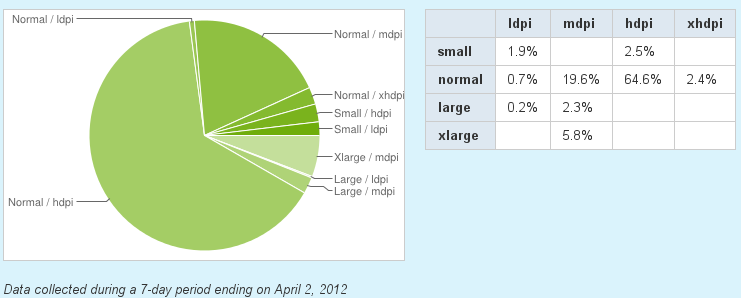
\includegraphics[width=3.5in]{densities.png}
\item Maybe just \texttt{xhdpi} if you're feeling brave.
\end{itemize}
\end{frame}

\begin{frame}{Directory structure}
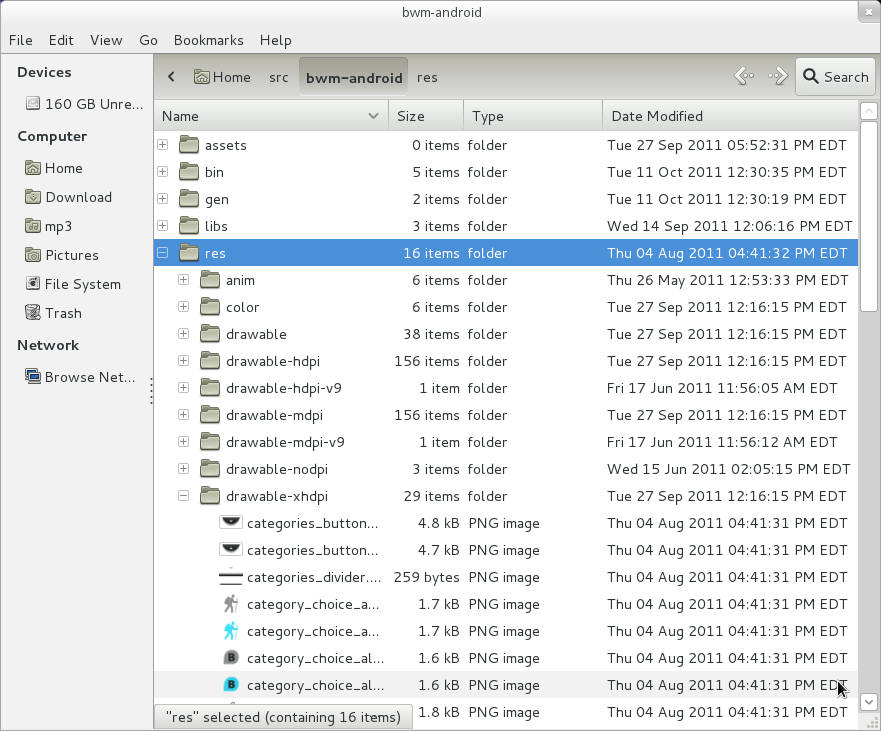
\includegraphics[width=3.5in]{nautilus.png}
\end{frame}

\begin{frame}{Additional qualifiers}
Rarely need to use more than one of these at a time, but they can be helpful:
\begin{itemize}
\item OS Version: \texttt{v9} etc.
\item Screen size: \texttt{small}, \texttt{medium} (phones);
  \texttt{large}, \texttt{xlarge} (tablets)
\item Language (and country): \texttt{en}, \texttt{es},
  \texttt{en-rCA}
\item Portrait/landscape: \texttt{port}, \texttt{land}
\item Many others, see SDK docs if interested.
\end{itemize}
Note! This applies not just to images but also, strings, layout files, etc.
\end{frame}

\begin{frame}{9-Patch Images}
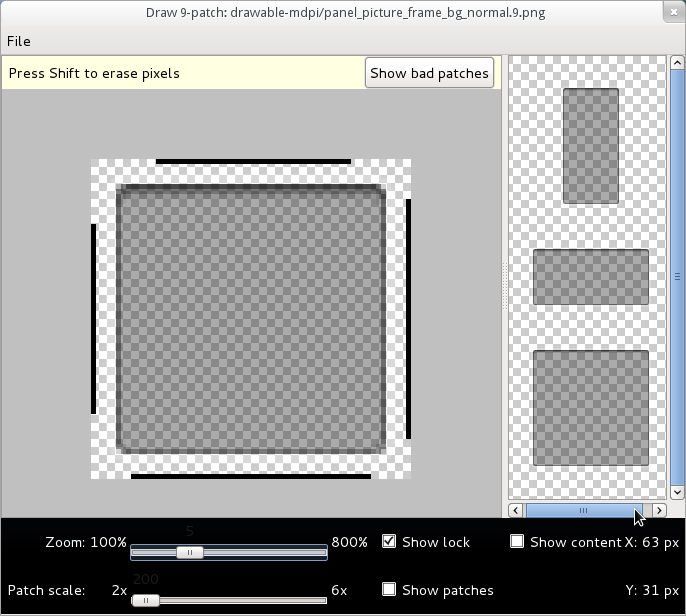
\includegraphics[width=3.25in]{draw9patch.png}
\end{frame}

\begin{frame}{Thank You}
Questions?
\end{frame}
\end{document}


